% Appendix B: Data lineage
\section{Data lineage}
\label{app:data-lineage}

\begin{figure}[ht]
\centering
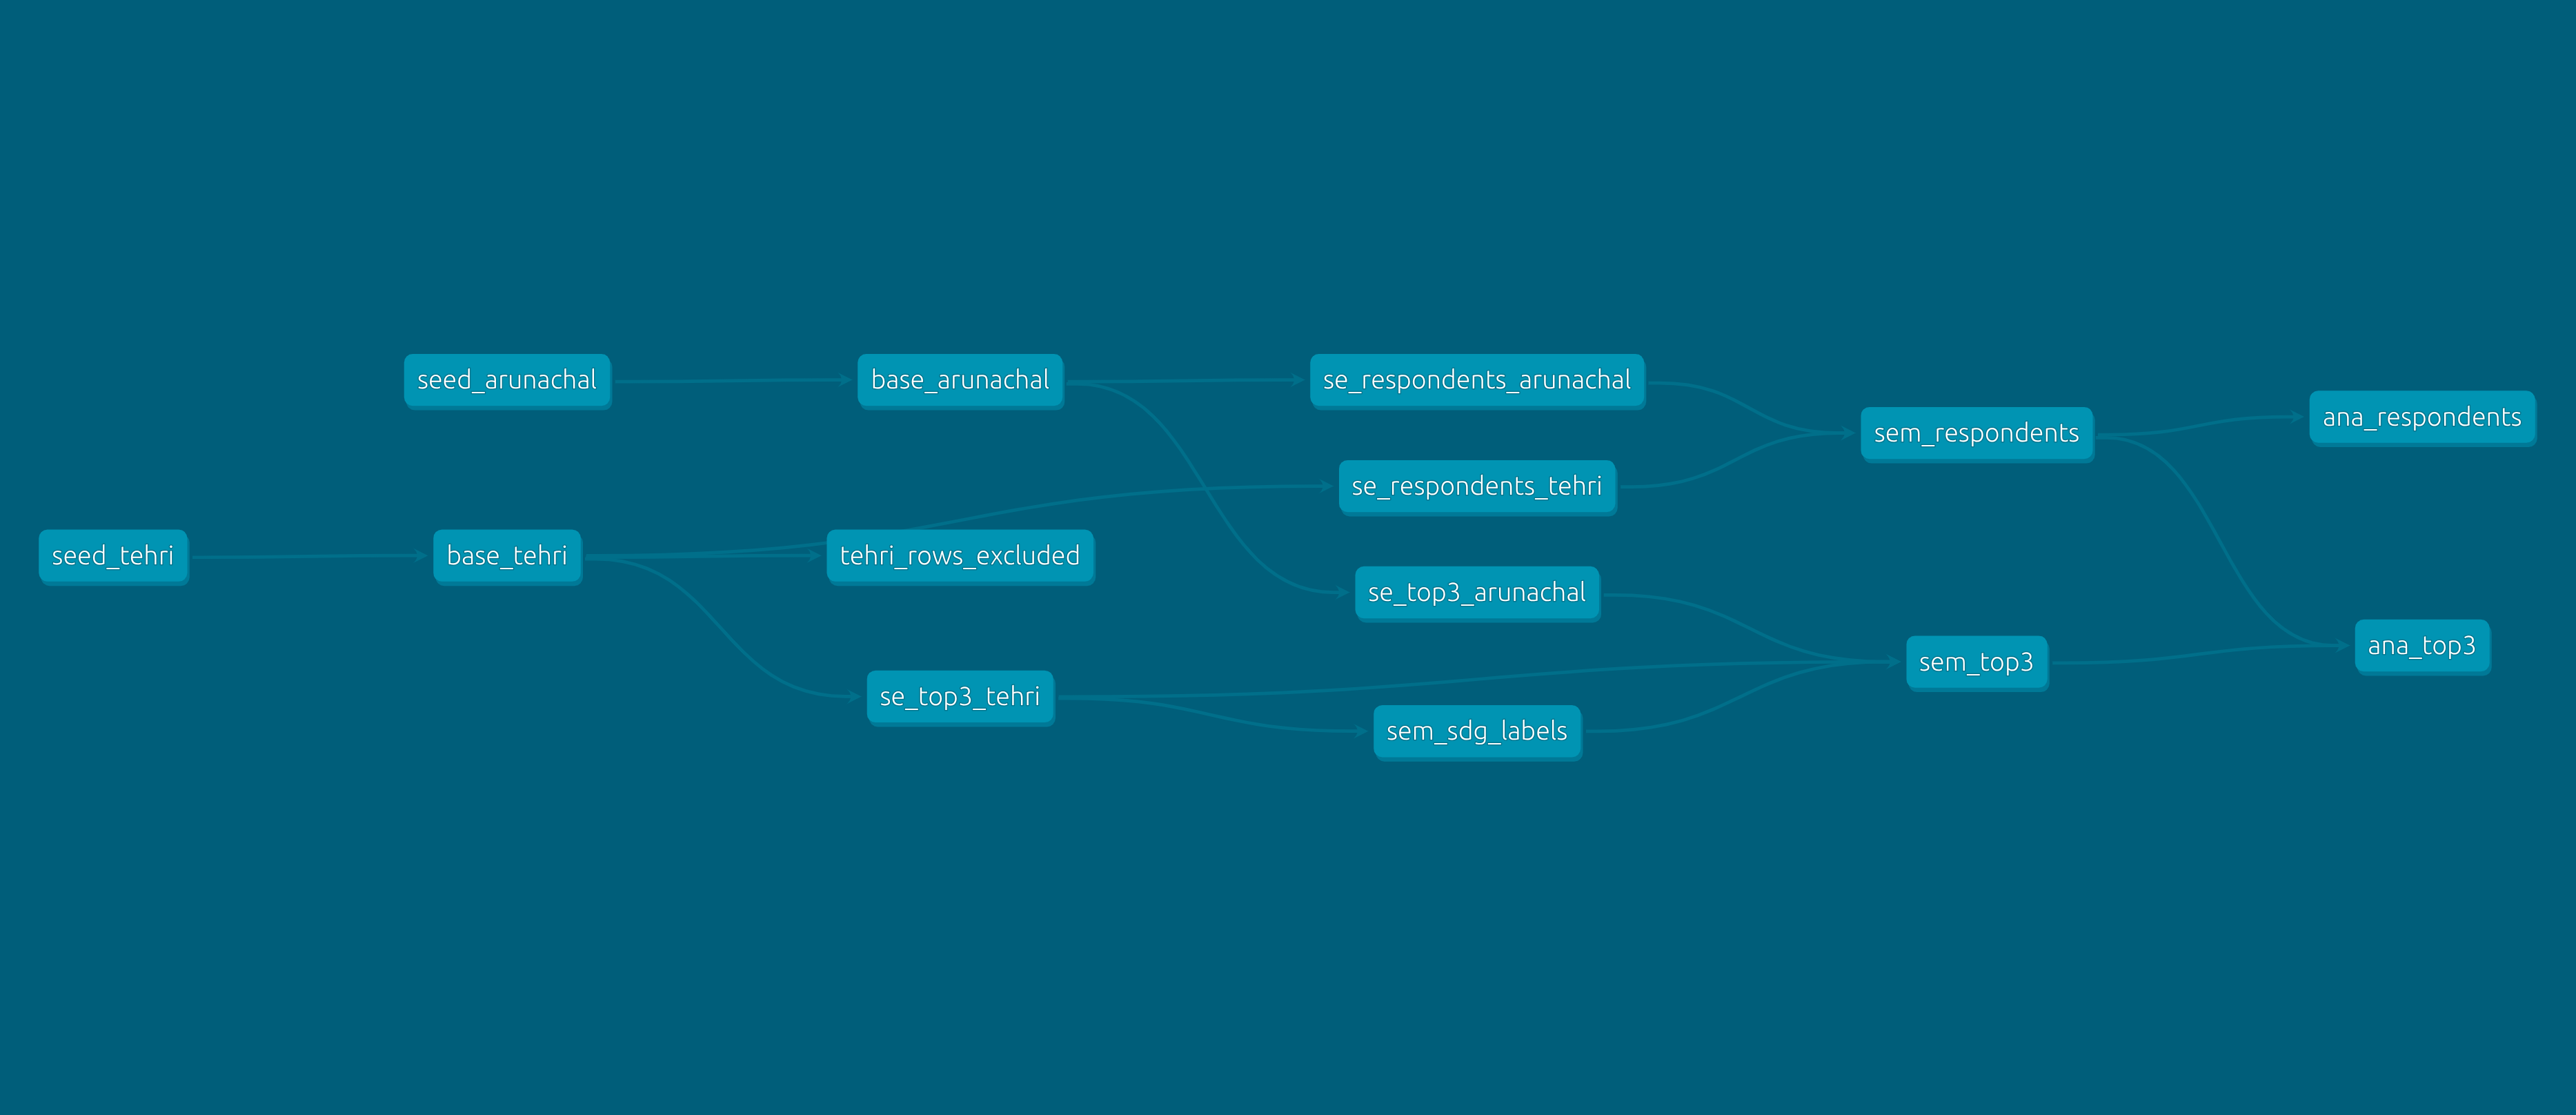
\includegraphics[width=\textwidth]{img/dbt-dag.png}
\caption{Data Build Tool (dbt) directed acyclic graph (DAG) showing the semantic layer structure from source entities through analytic models.}
\label{fig:dbtdag}
\end{figure}

\subsection{Source data and transformation overview}

The giveadam project begins with two regional survey datasets stored in \texttt{raw\_data/}. These datasets required integration across different formats: CSV files \cite{csv_rfc} from Arunachal Pradesh and Excel exports from the Kobo Toolbox \cite{kobo_toolbox} platform for the Tehri region. 

To unify these disparate sources, we implemented a comprehensive data transformation pipeline using the Data Build Tool (dbt) \cite{dbt_core,dbt_duckdb} within the \texttt{dbt\_project/} directory. The complete repository architecture supporting this pipeline is detailed in Section~\ref{sec:repository-arch}.

\subsection{Pipeline architecture and processing}

The transformation pipeline consists of SQL scripts \cite{sql}, automated tests, and comprehensive documentation that convert raw survey data into analysis-ready formats. A significant challenge involved extracting relevant columns from the complex Kobo export structure. We developed a dedicated R script \cite{r_core,tidyverse} (\texttt{scripts/tehri-cols.R}) to identify and map survey questions to data columns, with results documented in \texttt{figure\_and\_tables/tehri\_columns.md} \cite{markdown}.

\subsubsection{Data quality assurance}

Our quality assurance process includes automated identification and exclusion of invalid responses. During processing, we identified and removed two test rows from the Tehri dataset that exhibited substantial missingness and clear indicators of being test data rather than genuine survey responses. This exclusion process is fully documented in \texttt{dbt\_project/analyses/tehri\_rows\_excluded.sql} and reflects the methodological transparency principles outlined in Section~\ref{sec:semantic-methodology}.

\subsection{Visual data flow representation}

Figure~\ref{fig:dbtdag} presents the directed acyclic graph (DAG) generated by dbt for the complete transformation pipeline. This visualization serves multiple purposes:

\begin{itemize}
    \item \textbf{Dependency mapping:} Each node represents a data model or transformation step, while edges show the flow of dependencies between them
    \item \textbf{Layer visualization:} The graph clearly demonstrates the four-layer semantic architecture described in Section~\ref{subsec:semantic-layers}
    \item \textbf{Quality assurance:} The DAG shows how data validation and testing are integrated throughout the transformation process
    \item \textbf{Reproducibility:} The complete lineage enables full reproduction of any analytic dataset from source data
\end{itemize}

This architectural approach ensures data integrity and methodological transparency while enabling efficient processing and clear stakeholder communication.

\subsection{Model catalog and validation}

Table~\ref{tab:dbt_models} provides a comprehensive catalog of all dbt models created within the \texttt{dbt\_project/}, organized by semantic layer. These models implement the semantic extension of dbt's standard layering approach detailed in Section~\ref{subsec:core-innovation}. Each model serves a specific role in the semantic transformation process, from preserving source context to enabling research-ready analysis.

The validation framework supporting these models is documented in Table~\ref{tab:dbt_tests}, which details the automated quality checks applied at each transformation stage. This combination of systematic modeling and rigorous testing ensures both computational efficiency and methodological rigor.

\begin{table}[!h]
\centering
\caption{\label{tab:dbt_models}Data Build Tool (DBT) models created by dbt\_project, ordered by observability layer.}
\centering
\fontsize{8}{10}\selectfont
\begin{tabular}[t]{>{\raggedright\arraybackslash}p{0.18\textwidth}>{\raggedright\arraybackslash}p{0.75\textwidth}}
\toprule
Model & Description\\
\midrule
\addlinespace[0.3em]
\multicolumn{2}{l}{\textbf{Analytic Models}}\\
\hspace{1em}\cellcolor{gray!10}{ana\_respondents} & \cellcolor{gray!10}{Cleaned and transformed respondents data for analysis.}\\
\hspace{1em}ana\_sdg & UN SDG labels and numbers as identifiers.\\
\hspace{1em}\cellcolor{gray!10}{ana\_sdg7} & \cellcolor{gray!10}{Dataset reporting if SDG 7 was prioritised in top 3 ranking by respondents, with respondent metadata.}\\
\hspace{1em}ana\_top3 & Top 3 analytical model for key metrics\\
\addlinespace[0.3em]
\multicolumn{2}{l}{\textbf{Semantic Models}}\\
\hspace{1em}\cellcolor{gray!10}{sem\_respondents} & \cellcolor{gray!10}{Each row represents one respondent in either the survey undertaken in Tehri or the survey undertaken in Arunachale Pradesh.}\\
\hspace{1em}sem\_sdg\_labels & This is a transformation table to integrate SDG labelling across the two survey datasets.\\
\hspace{1em}\cellcolor{gray!10}{sem\_top3} & \cellcolor{gray!10}{Each row a ranking of top 3 SDG priorities, by one respondent from either the Tehri or Arunachal survey. In particular this step ensures that the SDG labels are harmonised across the two surveys.}\\
\hspace{1em}sem\_top3\_arunachal\_long & Long format of top 3 SDG rankings from Arunachal Pradesh respondents.\\
\hspace{1em}\cellcolor{gray!10}{sem\_top3\_tehri\_long} & \cellcolor{gray!10}{Each row represents a respondent's ranking of their top 3 UN Sustainable Development Goals (SDGs) for Tehri, India.}\\
\addlinespace[0.3em]
\multicolumn{2}{l}{\textbf{Source Entity Models}}\\
\hspace{1em}se\_respondents\_arunachal & Each row represents a respondent from Arunachal Pradesh.\\
\hspace{1em}\cellcolor{gray!10}{se\_respondents\_tehri} & \cellcolor{gray!10}{Each row represents a respondent from Tehri.}\\
\hspace{1em}se\_top3\_arunachal & Each row represents a respondent's ranking top 3 UN Sustainable Development Goals (SDGs) for Arunachal Pradesh, India. These data are extracted in wide format from the original survey data preserving labelling for data validation.\\
\hspace{1em}\cellcolor{gray!10}{se\_top3\_tehri} & \cellcolor{gray!10}{Each row represents a respondent's ranking of their top 3 UN Sustainable Development Goals (SDGs) for Tehri, India. These data are extracted in wide format from the original survey data preserving labelling for data validation.}\\
\addlinespace[0.3em]
\multicolumn{2}{l}{\textbf{Base Models}}\\
\hspace{1em}base\_arunachal & Raw data from survey in Arunachal Pradesh, collected by Dr Garima Gupta. Each row represents the survey responses of a single respondent. This step loads the data into the pipeline and establishes an identifier for each respondent. Only top 5 ranking and age and gender in these data, an extraction from the full arunachal dataset which is not available due to institutional restrictions. For this pipeline the top 3 rankings are extracted for analysis.\\
\hspace{1em}\cellcolor{gray!10}{base\_tehri} & \cellcolor{gray!10}{Raw data from survey in Tehri, collected by Dr Garima Gupta. Each row represents the survey responses of a single respondent. This step loads the data into the pipeline and establishes an identifier for each respondent. See `raw\_data/tehri\_cols.md` for details on all questions included in this dataset.}\\
\bottomrule
\end{tabular}
\end{table}
